\documentclass{article} % For LaTeX2e
\usepackage{nips15submit_e,times}
\usepackage{hyperref}
\usepackage{url}
\usepackage{graphicx,float,wrapfig}
%\documentstyle[nips14submit_09,times,art10]{article} % For LaTeX 2.09


\title{Applying Convolutional Neural Networks (CNNs) for Decoding fMRI Images}


\author{
Dong Hyun Choi \\
Department of Electrical and Computer Engineering\\
Carnegie Mellon University\\
Pittsburgh, PA 15213 \\
\texttt{donghyuc@andrew.cmu.edu} \\
\And
Yongjin Cho \\
School of Computer Science \\
Carnegie Mellon University \\
Pittsbrugh, PA 15213\\
\texttt{ycho1@andrew.cmu.edu} \\
}

\newcommand{\fix}{\marginpar{FIX}}
\newcommand{\new}{\marginpar{NEW}}
\def\code#1{\texttt{#1}}

\nipsfinalcopy % Uncomment for camera-ready version

\begin{document}


\maketitle

\begin{abstract}
We did what on which data set (using CNNs to decode 3-D image and predict word based on brain image). Our network looks like what. Some additional tricks we used are what. Our performance was what (comparing with baseline logistic regression classifier).
\end{abstract}

\section{Introduction}

Functional Magnetic Resonance Imaging (fMRI) is a brain imaging technology that enables us to know which part of the brain is active at any moment of a given task. Beyond trying to identify which brain region relates to certain tasks, there have been numerous attempts at trying to interpret the brain's activation state given the fMRI of itself. Specifically, Mitchell et al \textcolor{red}{[X]} has showed that machine learning algorithms could be used to predict what the brain was thinking of based on fMRI images depicting voxel activations. Further researchers, such as Ramish \textcolor{red}{[X]}, have also tried at developing cross-subject interpretation of fMRI images by using cross-subject clustering for improving the accuracy.

Convolutional Neural Network (CNN) is a recent technology that has shown good performance in various image analysis tasks such as image recognition and video recognition. Therefore, we attempt to use CNN as our main model in this paper to infer the state of the brain from a set of fMRI images. Though the task of inferring the brain's state from fMRI images could be regarded as a simple extension of previous image classification examples, the fact that fMRI images are 3-dimensional and that fMRI images across people can be different for the same task provides various challenges. For example, the voxels being activated while thinking of a certain object will differ depending on the person being inspected. We have chosen CNN as our model because we believe that CNNs will be able to extract general features from brain images that will help at providing better interpretation across all human subjects.

In order to see the relative performance of our CNN model, we first implement two baseline approaches: a logistic regression model and an artificial neural network model. We then compare the results of the baseline approaches to those of the CNN based approach and explain what could be the cause of the difference in those performances. 

For this midterm report, we include the details of our completed baseline approaches and the prototype of our CNN model. We also explain about the base dataset, how feature extraction was done from the dataset, the structures of our models, and the various problems that we've approached. We finish the paper by showing the performances of the different approaches and the project direction for the rest of the semester.  

\newpage
\section{Dataset}

\subsection{Base Dataset}

The base dataset includes nine sets of fMRI images, where each set corresponds to each unique human subject. Each image was taken while showing the subject a line drawing of one of the 60 concrete objects across 12 semantic categories. The set of objects were shown six times in random order, creating a total of 360 trials per subject.
%%%
The fMRI image was preprocessed to MNI template brain image and further normalized into MNI space and resampled to 3 by 3 by 6 $mm^3$ voxels.

This dataset is organized into nine separate files, where each file contains data for a single subject. The format of each file is as the following:
\begin{itemize}
	\item \textbf{META} : contains identifier of subject, number of trials, number of voxels activated for the subject during the entire trial, dimension of 3-dimensional coordinates of voxels, mapping info from voxel coordinate to voxel column in data, and inverse mapping info. 
	\item \textbf{INFO} : contains word (stimulus), semantic category of the stimulus, and the number of the stimulus has been presented to the subject.
	\item \textbf{DATA} : contains vectors of voxels for each of 360 trials. For each trial, there is a 1 by V voxel vector, where V is provided in \textbf{META} as nvoxel
\end{itemize}
%%%

\subsection{Preprocessed Dataset}

For our purpose of training the baseline models, the base dataset had to be preprocessed due to the irregularity of the number of voxels across all subjects. As the number of activated voxels for each subject were independent from one another, each image was first flattened into a $1-by-n$ feature vector, where $n$ is the number of activated voxels each person had, and then normalized it so that all vectors could have the same dimension $n'$. The value of $n'$ was chosen by the maximum number of voxels there could be inside one fMRI image. This could be determined from the meta info \code{dimx}, \code{dimy}, and \code{dimz} that states the range of each dimension. When normalizing each vector, the \code{colToCoord} meta info was used to map each value in the $1-by-n$ vector to the new $1-by-n'$ vector. As $n' > n$, all points where no \code{colToCoord} was given were initialized to be zero. This eventually created a default set of feature vectors with a dimension of $51 \cdot 61 \cdot 23 = 71553$.
%Since we were provided the range of x,y,z coordinates of voxels in meta field, for each data instance, we initialized 3-d zero array of dimension (dimx, dimy, dimz), filled corresponding voxel value by using colToCoord info, and flattened the 3-d array, resulting into 1 by dimx*dimy*dimz vector. Thus, the basic feature is to represent each data instance as 1 by dimx*dimy*dimz vector. 

The second set of feature vectors was extracted by applying Principal Component Analysis (PCA) to the data matrix $X$, where $X$ was created by stacking the feature vectors vertically as column rows. Thus, the $i_{th}$ row in $X$ would be a $1-by-71553$ vector depicting the $i_{th}$ fMRI image from the original dataset. We used only the first 200 principal components and projected all data onto those components. In this case, each data instance's feature became a $1-by-200$ vector.

The last set of feature vectors was extracted by applying Linear Discriminant Analysis (LDA) to the same data matrix $X$ that was used for applying PCA. Class labels were also provided along with the data when applying LDA, where each class label was a mapping from the 60 words that subject was tested for to a number within the range of 0 to 59. This reduced the dimension of each feature vector from the original 71553 to 59.

\section{Baseline Approaches}

The task for each baseline model is to predict the word of the object that the subject was being shown when the fMRI image was taken. A random choice would provide an accuracy of $1.67\%$, which is the probability of choosing one out of 60 possible candidates. All three types of feature vectors were tested to see which set of feature vectors would yield the best accuracy and performance.

\subsection{Logistic Regression}

As the first baseline approach, we implemented multinomial logistic regression.  
The L2 regularization was used, and the gradient descent was used for optimization of parameters. 

For evaluation of the classifier's performance, we did nine evaluations such that in $i$ th evaluation, we used all the data from subject except $i$th subject's data for training and evaluated the accuracy of classifier for the unused $i$th subject's data. And we took average of those nine accuracies. 

For Logistic Regression classifier, we used all three types of features described in section 2.2. The results are provided in section 7 along with performances of other approaches. 

\subsection{Artificial Neural Network}

As the second baseline approach, we implemented Artificial Neural Network (ANN) with two hidden layers, each layer having 1024 hidden units, and RELU activation unit. 

For evaluation of the classifier's performance, we did nine evaluations such that in $i$ th evaluation, we used all the data from subject except $i$th subject's data for training and evaluated the accuracy of classifier for the unused $i$th subject's data. And we took average of those nine accuracies. 

For ANN classifier, we used two types of features, LDA and PCA, described in section 2.2. The results are provided in section 7 along with performances of other approaches. When we used the first type feature where each data instance is 1 by xdim*ydim*zdim for each instance, each data instance becomes a sparse vector with nonzero elements ratio being approximately $\frac{1}{3}$. Having very sparse vector representation for each data instance resulted in underflow in back-propagation within ANN, thus we experimented ANN classifier only with PCA and LDA features.  

\section{CNN Architecture}

We apply the same task that was used for the baseline models to the CNN model, which was to predict the word from the fMRI image. Three different structures are proposed in order of expected performance improvements. For the first two structures, we use the same CNN structure which consists of two convolutional layers, two pooling layers, and a fully connected layer at the end. ReLU units were chosen to represent each hidden layer, as ReLUs are believed to --- \textcolor{red}{[X]}. Hyperparameters were set to start with a stride of two $(S=2)$, a receptive field size of 5 x 5 $(F=5)$, a slice depth size of 16 $(K=16)$, and a padding size of zero $(P=0)$. These initial hyperparameters are based on the CNN structure that is most popularly used for MNIST demos \textcolor{red}{[X]}, as the image dimensions of our brain images (23-by-61, 23-by-51, or 61-by-51) were not significantly different from that of MNIST images (28-by-28). Only the first proposed structure has been fully tested at the time of this report.

\subsection{Ensemble of CNNs With Voting}

As our CNN structure was created to mainly deal with 2-dimensional images, the original 3-dimensional data was split into sets of 2-dimensional images along each $x$, $y$, and $z$ axis to match the input format that the model requires. Three separate CNN models were created for data from each axis, and the final prediction was determined by the vote from all three. Figure 1 shows the ensemble of the three CNN models. When all three models predicted different labels, the prediction with the strongest confidence rate was chosen as the tie breaker.

\begin{figure}[H]
	\centering
	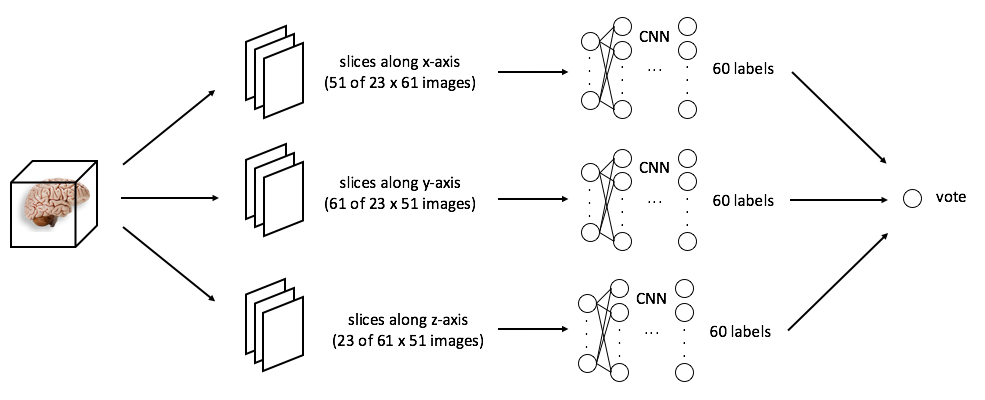
\includegraphics[height=0.26\textheight]{./img/cnn_proto_a.png}
	\caption{Structure of ensemble of CNNs by predicting the final label through voting.}
\end{figure}

However, each CNN model reported very low accuracy for their label prediction, where the accuracy was no different from choosing the label at random. As each CNN model was not performing reasonably, the end vote was also no different from choosing any label. We provide some analysis of the possible causes of this performance at the results section of this paper.

\subsection{Ensemble of CNNs With Connected End Layers}

Talk about it.

\begin{figure}[H]
	\centering
	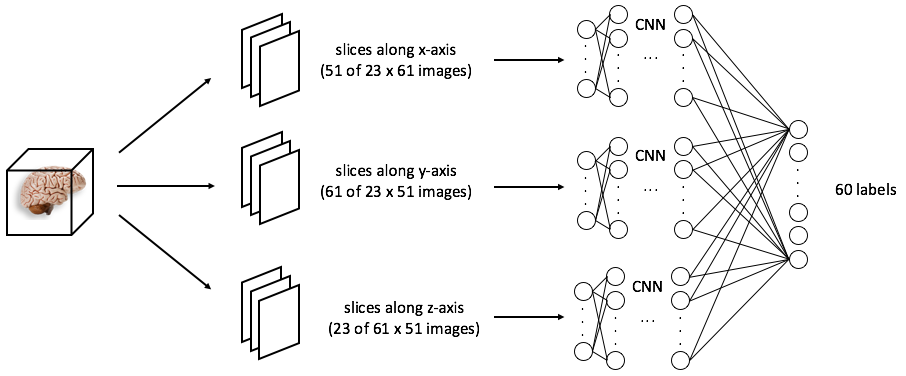
\includegraphics[height=0.26\textheight]{./img/cnn_proto_b.png}
	\caption{Structure of ensembles of CNNs by connecting all end layers.}
\end{figure}

\subsection{3-dimensional Convolutional Layers}

Talk about it.

\begin{figure}[H]
	\centering
	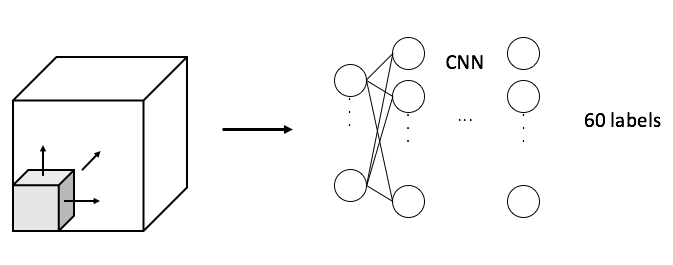
\includegraphics[height=0.2\textheight]{./img/cnn_proto_c.png}
	\caption{Structure of a CNN with 3-dimensional convolutional layers.}
\end{figure}

\section{Results}

Show table. Compare accuracies based on different settings. Compare with baseline and random choice.
\begin{table}[H]
\centering
\caption{Logistic Regression}
\label{my-label}
\begin{tabular}{|c|c|}
\hline
\textbf{Feature Type} & \textbf{Accuracy} \\ \hline
Basic                 &                   \\ \hline
PCA                   &                   \\ \hline
LDA                   &                   \\ \hline
\end{tabular}
\end{table}

\begin{table}[H]
\centering
\caption{Artificial Neural Network}
\label{my-label}
\begin{tabular}{|c|c|}
\hline
\textbf{Feature Type} & \textbf{Accuracy} \\ \hline
PCA                   &                   \\ \hline
LDA                   &                   \\ \hline
\end{tabular}
\end{table}

\begin{table}[H]
\centering
\caption{Convolutional Neural Network}
\label{my-label}
\begin{tabular}{|c|c|}
\hline
\textbf{Feature Type} & \textbf{Accuracy} \\ \hline
Basic                 &                   \\ \hline
PCA                   &                   \\ \hline
LDA                   &                   \\ \hline
\end{tabular}
\end{table}

\subsection{Qualitative Evaluation}

Maybe talk about sample images.

\section{Direction for the Rest of Semester}

Our results show something. Some possible improvements might be something.

\section*{References}

\small{
[1] Alexander, J.A. \& Mozer, M.C. (1995) Template-based algorithms
for connectionist rule extraction. In G. Tesauro, D. S. Touretzky
and T.K. Leen (eds.), {\it Advances in Neural Information Processing
Systems 7}, pp. 609-616. Cambridge, MA: MIT Press.

[2] Bower, J.M. \& Beeman, D. (1995) {\it The Book of GENESIS: Exploring
Realistic Neural Models with the GEneral NEural SImulation System.}
New York: TELOS/Springer-Verlag.

[3] Hasselmo, M.E., Schnell, E. \& Barkai, E. (1995) Dynamics of learning
and recall at excitatory recurrent synapses and cholinergic modulation
in rat hippocampal region CA3. {\it Journal of Neuroscience}
{\bf 15}(7):5249-5262.
}

\end{document}